\section{Subsistema: Localização e Informações}

  \subsection{Adaptação do Ambiente}

  Sabendo que o plantio do morango utiliza o arranjo de fileiras,
  optou-se por uma abordagem baseada na utilização de sensores, juntamente a um 
  algoritmo capaz de processar os dados referentes à distância do veículo em 
  relação à cada fileira, posicionada sempre à direita.
  Basicamente o veículo utilizará as fileiras como guia, de forma a realizar a 
  coleta de dados em todas as fileiras da plantação. Com a finalidade de viabilizar essa 
  solução serão necessárias algumas adaptações no terreno conforme descreve a figura \ref{fig:adapt}. 

  \begin{figure}[!htbp]
  \begin{center}
  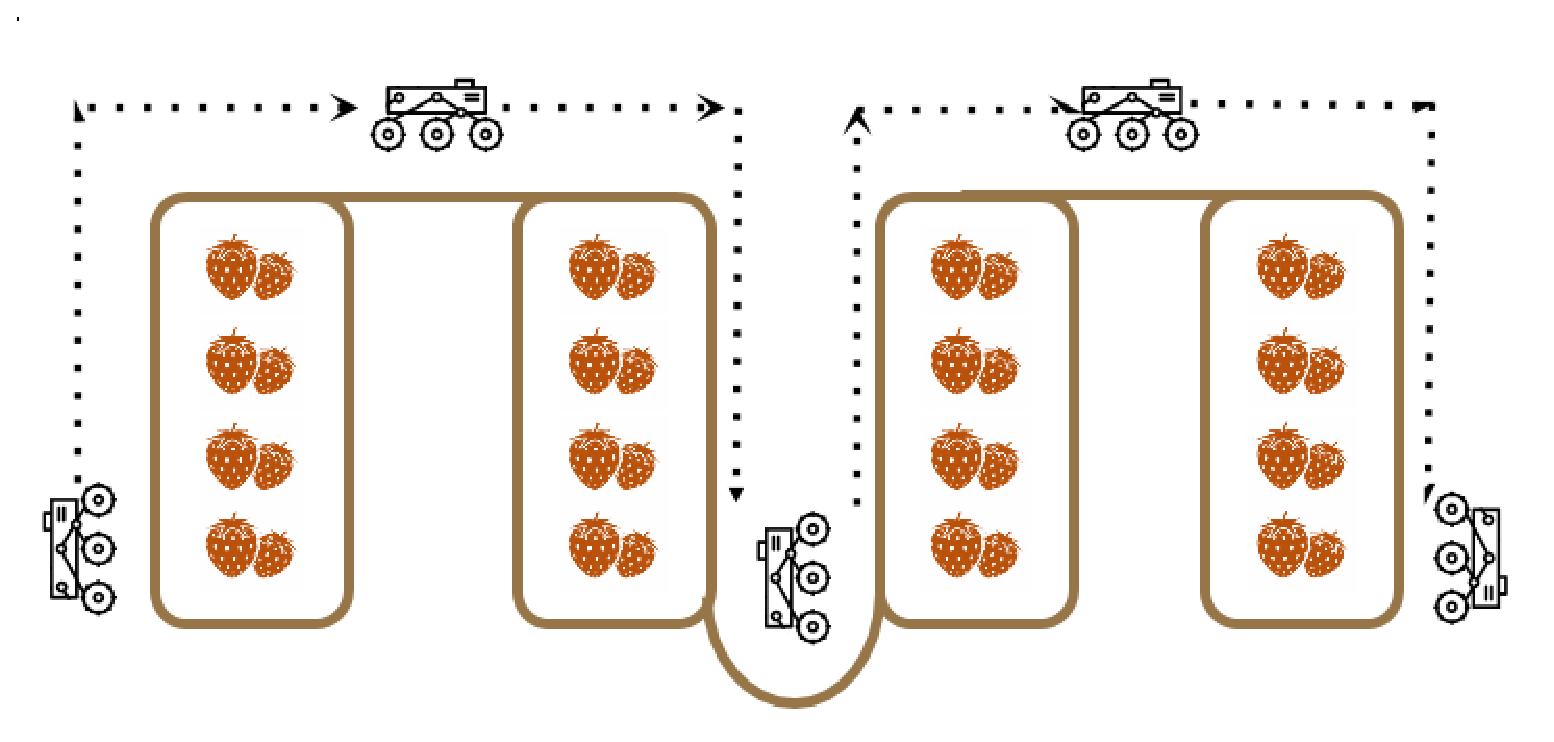
\includegraphics[width=.7\textwidth]{figuras/adapt.eps}
  \caption{\label{fig:adapt}Adaptação do ambiente.}
  \end{center}
  \end{figure}

  \subsection{Sensoriamento: Localização}

  Para as medições referentes à distância foram considerados sensores baseados
  em dois tipos de princípios, ultrassom e infravermelho. Inicialmente a opção
  baseada em ultrassom se mostrou mais adequada, porém foi possível perceber
  que os principais sensores comerciais que se baseavam nesse princípio
  possuíam uma faixa de detecção bastante reduzida. Sendo assim, foi
  escolhido um sensor de proximidade baseado em infravermelho apresentado
  na figura~\ref{fig:infrared}.

  \begin{figure}[!htbp]
  \begin{center}
  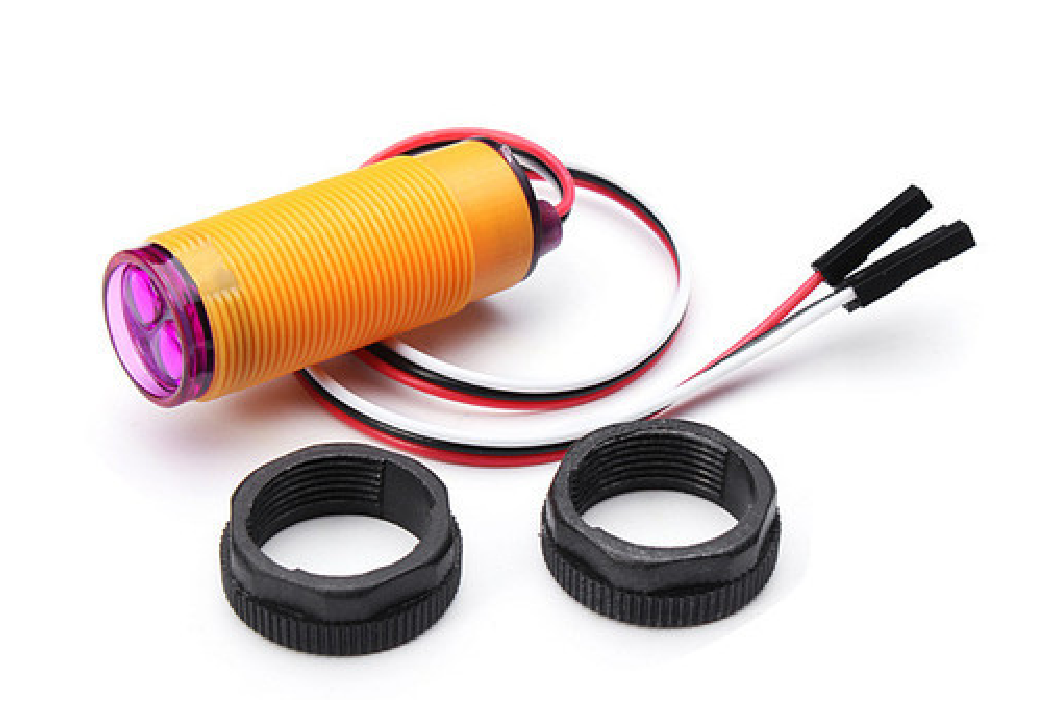
\includegraphics[width=.7\textwidth]{figuras/infrared.eps}
  \caption{\label{fig:infrared}Sensor de proximidade infravermelho.}
  \end{center}
  \end{figure}

  O princípio de funcionamento deste sensor é o princípio da triangulação.
  Um feixe de luz é emitido por um diodo laser ou um LED infravermelho.
  Ao ser refletido por um objeto, esse raio é detectado por um PSD
  (\textit{Position Sensing Device} -- Dispositivo de Monitoramento de Posição).
  De acordo com a distância do objeto que refletiu a luz, esse raio incide
  de modo diferente no PSD. A figura~\ref{fig:infrared_func} ilustra o
  princípio da triangulação.

  \begin{figure}[!htbp]
  \begin{center}
  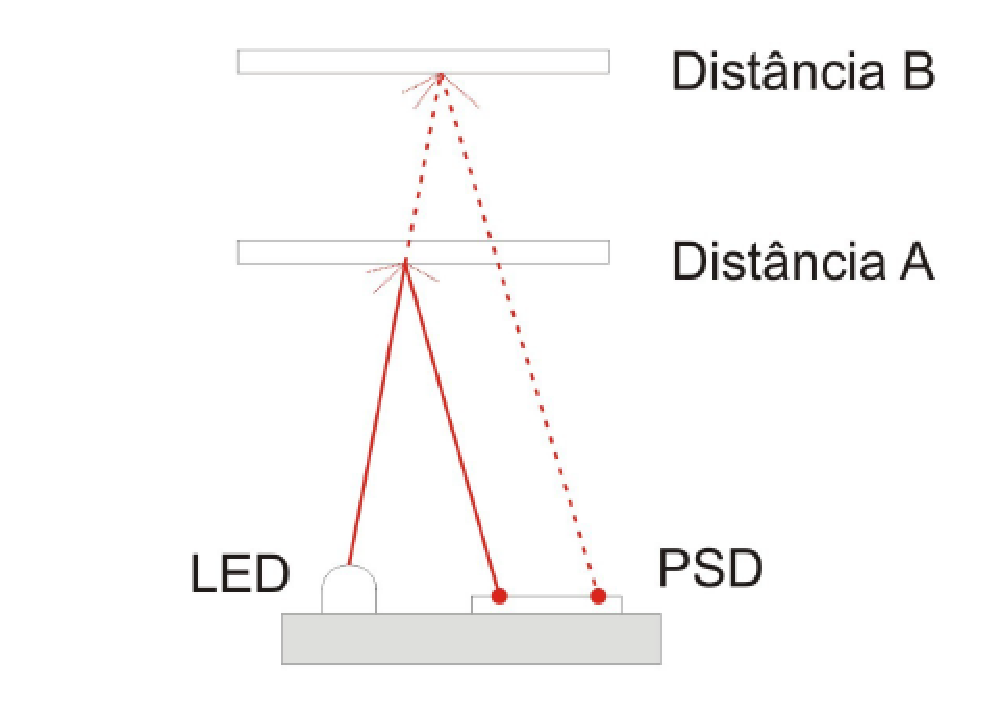
\includegraphics[width=.7\textwidth]{figuras/infrared_func.eps}
  \caption{\label{fig:infrared_func}Princípio da triangulação.}
  \end{center}
  \end{figure}

  A escolha do elemento foi motivada pela capacidade de detecção
  de proximidade ser adequada para o funcionamento do algoritmo
  de localização, mais especificamente entre 3 e 80cm.  Além disso,
  este elemento apresenta pouca interferência com a luz visível e
  possui um interfaceamento simples com um microcontrolador.

  \subsection{Unidade de Processamento}

  A unidade de processamento escolhida foi o Raspberry Pi B+,
  devido a sua robustez. Esta unidade conta com o microprocessador
  BCM2835 da Broadcom, que é baseado no ARM1176JZFS com clock de
  700MHz e modo de baixo consumo, uma GPU Dual Core VideoCore
  IV\textregistered, SDRAM de 512MB, 4 portas USB, 1 porta RJ45
  (Ethernet), 1 porta HDMI e 40 pinos para GPIO~\cite{raspref}

  Esta unidade terá um sistema operacional Linux embarcado e
  servirá para armazenar os dados obtidos pelos sensores, para
  as decisões do controle do veículo, para o armazenamento dos
  parâmetros iniciais de posicionamento e pontos de coleta de
  dados, assim como para o cálculo do posicionamento e passagem
  dos dados para a base.

  \begin{figure}[!htbp]
  \begin{center}
  \includegraphics[width=.7\textwidth]{figuras/raspberry.eps}
  \caption{\label{fig:raspberry}Raspberry Pi B+.}
  \end{center}
  \end{figure}

  \subsection{Algoritmo de Localização}

 \begin{itemize}

 \item Processamento de Imagens

  Processamento de imagens consiste em uma técnica para a análise de dados
  multidimensionais, que permite manipular e tratar imagens com objetivo de
  obter informações e melhorar as características visuais da imagem.
  A primeira etapa consiste em adquirir uma imagem, por exemplo,
  através de uma câmera digital, de um scanner laser, de um ultrassom,
  de um ressonador magnético, ou por qualquer outro meio. Após a captura,
  uma imagem precisa ser representada de forma apropriada para tratamento
  computacional, ou seja, sua representação se dará como uma função
  bidimensional ou tridimensional. Feito isso, inicia-se o pré-processamento
  da imagem. Nessa etapa a imagem passa por um processo de filtragem,
  no qual são eliminados os ruídos, que podem ser obtidos durante a
  captura da imagem, melhorando assim a qualidade e permitindo uma melhor
  discriminação dos objetos presentes na mesma.

  Pelo curto tempo destinado ao desenvolvimento do projeto e a falta de
  conhecimento da equipe sobre o assunto, a escolha por processamento de
  imagens acabou sendo descartada pelo seu alto grau de risco ao projeto.

 \item Localização por meio GPS

  O sistema de posicionamento global (GPS) é uma tecnologia
  para navegação em ambientes externos. O GPS foi desenvolvido
  pelo Departamento de Defesa Americano, sendo composto por um conjunto
  de satélites que transmitem um sinal de rádio-freqüência codificado.
  Usando-se métodos de trilaterização avançados, receptores no solo podem
  medir as suas posições baseado no tempo de viagem dos sinais de
  rádio-freqüência dos satélites, permitindo o cálculo da latitude,
  longitude e altitude do receptor.

  O principal problema de se usar marcos naturais do ambiente na
  navegação é detectar e combinar as características dos marcos
  a partir das informações dos sensores. A escolha natural do sensor
  para esta tarefa é a visão computacional. A maior parte dos marcos
  naturais do ambiente baseados em visão são longas bordas verticais,
  como portas, junções de paredes e luzes no teto.

  Pelo local da plantação ser um ambiente de tamanho de visibilidade
  baixa e possuir características específicas da plantação, a localização
  por GPS se torna insatisfatória para o projeto, uma vez que erros
  referentes à precisão podem acarretar em um comprometimento da plantação
  por parte do veículo.


 \item Localização por Sensoriamento

  As abordagens estudadas que podem resolver o problema da localização
  basearam-se no sensoriamento infravermelho e ultrassônico.
  Dado as condições da lavoura de morango ambos poderiam ser
  aplicados como um problema referente à Wall follower.
  
  Wall follower é a regra mais conhecida para percurso em labirintos,
  também conhecido como regra da mão direita ou esquerda.
  Ela é válida para percursos conexos, onde todas as paredes são
  ligadas entre si, mantendo a mão próxima a parede do labirinto em
  que se inclui, garantindo assim que o corpo não se perca e finalize
  o percurso. O principal problema desta regra ocorre quando um percurso
  possui loops de passagens que projetem uma trajetória sem fim.

 \item Solução adotada: \textit{Wall Follower}

  A solução adotada para o projeto baseou-se na utilização de sensores
  infravermelho, pois atendiam os requisitos com maior simplicidade,
  menor custo técnico e computacional.
  
  Todavia, devido as soluções adotadas para tração, movimentação das
  rodas e perfuração (realizada somente pelo lado direito do veículo),
  serão necessárias algumas modificações no ambiente de plantio para modelagem
  do sistema como um cenário “Wall Follower” citado acima.
  
  Para que o veículo seja capaz de percorrer todas as fileiras sem passar
  pelo mesmo caminho de maneira redundante, foi pensada a adição de
  estruturas à lavoura para montar uma espécie de circuito. O esquemático
  abaixo representa a estrutura da lavoura e o caminho a ser percorrido pelo
  veículo que irá seguir sempre a parede à sua direita até completar todo o
  percurso.

  Para a escolha do material ponderou-se necessidade de um material
  barato e de fácil instalação/manuseio. Desta forma, o plástico e
  a madeira foram os materiais escolhidos para compor os obstáculos
  que irão ajudar o veículo a percorrer o trajeto.

\end{itemize}

  \subsection{Armazenamento dos Dados}

  Para o armazenamento de dados foi escolhido um cartão de memória
  Micro SD de 8GB da Sandisk. Sua escolha foi motivada devido à
  necessidade de um dispositivo de armazenamento portátil, capaz de
  armazenar os dados adquiridos a partir dos sensores para a posterior
  análise. Além disso, a placa microprocessadora escolhida oferece
  suporte para cartão de memória, dispensando o uso de um módulo avulso
  para a realização das operações de armazenamento. A figura~\ref{fig:sdcard}
  apresenta o cartão de memória. 

  \begin{figure}[!htbp]
  \begin{center}
  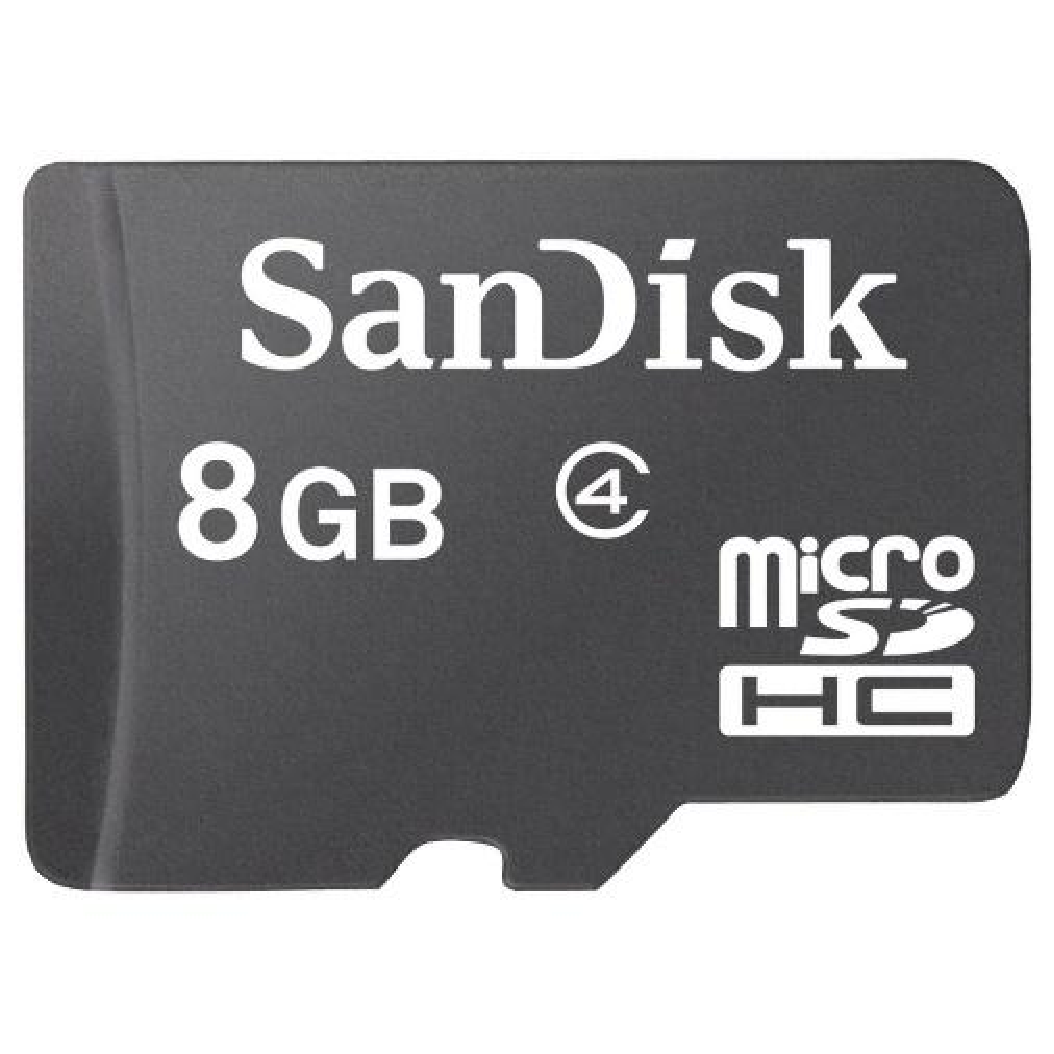
\includegraphics[width=.5\textwidth]{figuras/sdcard.eps}
  \caption{\label{fig:sdcard}Cartão de memória.}
  \end{center}
  \end{figure}

  Os dados serão armazenados no cartão de memória da Raspberry Pi
  em um arquivo no formato CSV (\textit{Comma Separated Value}). Os dados
  serão dispostos em colunas com a seguinte ordem: posição da medição
  em metros, umidade do solo, umidade relativa do ar e temperatura do
  ambiente.
  Os dados dispostos desta maneira facilitam o processamento e
  análise posterior, assim como sua apresentação gráfica para
  o operador.

  \subsection{Leitura das Informações}

  Uma parte importante do o projeto consiste na apresentação dos
  dados para o gestor da lavoura. Foi definido que para esse fim,
  a solução será uma aplicação, feita na linguagem Ruby com o
  auxílio do \textit{framework} Rails, que é um \textit{framework}
  para desenvolvimento de aplicações web.
  A escolha de desenvolver utilizando-se essa linguagem junto a
  esse \textit{framework} foi feita com base na facilidade que essa
  tecnologia fornece para o desenvolvimento e com base na experiência
  da equipe responsável pelo desenvolvimento da aplicação, visto que
  todos os desenvolvedores já possuem experiência com a tecnologia
  escolhida.
  
  Em concordância com os requisitos estabelecidos, essa aplicação
  permitirá o upload do arquivo CSV gerado pelo veículo, dentro de
  uma área restrita da aplicação, disponível apenas após a realização
  do login.
  Após a realização do upload, o usuário possuirá a opção de visualizar
  os dados de forma gráfica, sendo que a visualização gráfica se dará
  com base em um heatmap (mapa de calor) para uma melhor representação
  da lavoura.
  Além da representação gráfica, o gestor da lavoura poderá obter
  esses dados em formato de relatório, sendo permitida sua
  exportação para um arquivo PDF (Portable Document Format).
